\documentclass{article}%
\usepackage[T1]{fontenc}%
\usepackage[utf8]{inputenc}%
\usepackage{lmodern}%
\usepackage{textcomp}%
\usepackage{lastpage}%
\usepackage{authblk}%
\usepackage{graphicx}%
%
\title{Genetic and epigenetic alterations are involved in the regulation of TPM1 in cholangiocarcinoma}%
\author{Thomas Miller}%
\affil{CNRS UMR 5203, INSERM U661, and Montpellier 1 \& 2 University, Institute of Functional Genomics, Montpellier, France, \newline%
    Laboratory for Diabetes Cell Therapy, Institute for Research in Biotherapy, University Hospital St{-}Eloi, Montpellier, France}%
\date{01{-}01{-}2013}%
%
\begin{document}%
\normalsize%
\maketitle%
\section{Abstract}%
\label{sec:Abstract}%
By JACQUELINE GRAZIER\newline%
STAFF WRITER\newline%
Defective murine macrophages of a certain type and of a different kind play roles in Francisella tularensis.\newline%
Unfortunately, the healthy immune system often fails to protect against this chronic illness and causes more than 1,000 additional deaths each year, including in the 150 or so Western Caesarean sections.\newline%
Often in men with breast cancer, macrophages act as a dysfunctional immune cell that disrupts normal cell cycles.\newline%
Genetic studies suggest macrophages are often responsible for hypochlorous acid levels (hypsis) by mistakenly activating another macrophage system.\newline%
This mouse version of LGS{-}T9{-}APNT3{-}RP{-}PRAPPS{-}CPSA is a mutant protein called CPCA, which controls the proliferation of muscle cells in this very rare disease.\newline%
Wondering why this mutant protein leads to tumor cell death, UC San Diego researchers discovered an intergroup of macrophages, positioned to help defend against skin cells.\newline%
Whats important is that they also could slow the production of the particular protein that suppresses muscle growth.\newline%
In the last 10 to 15 years, the UC San Diego Cancer Research Institute has been working on non{-}DNA{-}based biomarkers that can really help us monitor immune function in the clinic, said senior author Genekhon Vital, M.D., Ph.D., UC San Diego Faculty Member.\newline%
He added: Weve been exploring the intersection of epigenetic, and genetic, elements for the past 15 years.\newline%
Weve shown that a gene called CPCA has a lot of gene activity in macrophages in patients with a metastatic cancer who also have knee or hip conditions like stenosis of the knee and hip joint.\newline%
Vital and his colleagues determined CPCA was activated in at least three macrophages that normally help fight the disease. These macrophages had extensive structural damage, and they had lived for longer periods in the body than normal macrophages, allowing them to be an important target for therapy.\newline%
We already had a mouse model with the disease, which was remarkably successful, Vital said. We needed to understand how the macrophages look from mouse populations to develop methods of isolating more human mollusks that have similar disease profiles.\newline%
Their serendipitous discovery was made with the recent launch of Francisella , a regional medical education initiative, which will focus on prostate cancer and help improve understanding of macrophage function in a specific setting such as nephrology.\newline%
Vital and his team already have begun to develop mouse models for this rare inflammatory condition and for other viral infections.\newline%
Osteoarthritis and ulcerative colitis, both of which affect blood vessels, are two indications of treatment based on protein therapy modulated by macrophages.\newline%
The UC San Diego researchers have also created a system for collaborating with colleagues at the University of Bristol in the U.K. to develop drug targets and biomarkers that respond to them.\newline%
We understand the importance of this genomic and molecular approach that were developing, Vital said. To me its critically important to understand diseases in diverse populations. When I was growing up it was human lymphoma that was the most obvious example.\newline%
Since many European cancers have similar genetic profiles to those diagnosed in their province of origin, the UC San Diego researchers believe it will be important to study how macrophages and key proteins could one day be integrated into new and better targeted treatments.

%
\subsection{Image Analysis}%
\label{subsec:ImageAnalysis}%


\begin{figure}[h!]%
\centering%
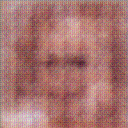
\includegraphics[width=150px]{500_fake_images/samples_5_7.png}%
\caption{A Black And White Photo Of A Black And White Photo}%
\end{figure}

%
\end{document}